\section*{Applicable Documents}

\begin{table}[H]
    \centering
    \resizebox{\columnwidth}{!}{
    \begin{tabular}{lll}
        \hline
        \textbf{Reference} & \textbf{Document Title} & \textbf{Issue/Release Date} \\
        \hline
        RD01 & ECSS-E-ST-31C Space Engineering & Issue 2, 2008/11/15 \\
        RD02 & ECSS-E-HB-31-01 - Space Engineering - Thermal design handbook - Part 1 to 16 & multiple \\
        RD03 & P. D.G. Gilmore, “Spacecraft Thermal Control Handbook: Fundamental Technologies”, ESA-TEC-MTT & 2002 \\
        \hline
    \end{tabular}
    }
\end{table}

\newpage

\section{Introduction}
The $^{\text{Po}}$Cat-Lektron Thermal Analysis is aimed to verify that all the components of the spacecraft
work in its operational temperature range during all mission phases. In order to develop
an accurate enough model, the following approach has been considered:

First, an isothermal solid cube will serve as an initial model. After that, models considering
radiation as the principal mode of heat transfer will provide more accurate results. Later
on, models considering both conduction and radiation as the main modes of heat transfer
will allow the needed characterization of the spacecraft to verify the thermal requirements
of each component.
\paragraph{}
In this document, the isothermal analysis and the radiation analysis of the $^{\text{Po}}$Cat
2 and $^{\text{Po}}$Cat3 satellites are presented.

The main objective of the isothermal analyses is to identify a passive thermal control
which maintains the spacecraft temperature in the correct behavior. In this case
, the evaluated technique is the use of different paints on the spacecraft surface.
\paragraph{}
As for the radiation analyses, they are aimed to validate the spacecraft thermal model
and verify its behavior under different heating environments.

\subsection{The \texorpdfstring{\textsuperscript{Po}}CCat-Lektron mission}

\subsubsection{Mission statement}

The $^{\text{Po}}$Cat-Lektron is a mission resulting from the IEEE OpenPocketQube Kit initiative, 
developed at the UPC NanoSat Lab. The mission has been selected in the 4th call of 
the ESA Fly Your Satellite! (FYS) program. The mission analysis presented corresponds 
to the $^{\text{Po}}$Cat-Lektron mission. It consist of two 1P PocketQubes, the PoCat-2 and the 
PoCat-3, developed as a part of the IEEE OpenPocketQube Kit. This mission aims to 
demonstrate the feasibility of PocketQube platforms for remote sensing applications.\cite{wiki}
\paragraph{}
The payloads on board of the PocketQubes are two passive radiometers to be use for 
RFI purposes on K and L bands. Apart from the remote sensing nature of the mission, 
this mission also aims to demonstrate the feasibility of the PocketQube platforms to 
create, manage and join Federated Satellite Systems. To do so, the FSS Experiment 
will be reproduced as a part of the experiments of the mission.

\subsubsection{Mission Objectives}

\begin{itemize}
    \item \textbf{Demonstration of Scientific Viability:} Demonstrate the feasibility of 
    conducting scientific missions using PocketQube platforms. To do so, the mission
    proposes collecting valuable RFI data through a K-Band and L-Band passive 
    radiometers (One for each PocketQube). The payloads will monitor interferences on 
    these bands. This data will facilitate enhanced detection and the generation of
    heatmaps indicating RFI distribution across the globe. In this experiment we aim
    to obtain data on the K-Band to see the impact on the atmospheric water vapor 
    measurements, and in the L-Band the interferences over the Position Navigation 
    and Timing (PNT) signals.

    \item \textbf{Satellite Federation Concept:} To establish and demonstrate that 
    PocketQube platforms can create, manage and join Federated Satellite System 
    (FSS). This proof of concept for this resource-limited platforms is based on 
    the reproduction of the FSS Experiment conducted at the UPC NanoSat Lab. The 
    demonstration consist on create a federation between 2 PocketQubes, in order 
    to download data. Previous missions such as the FSS-Cat from the UPC NanoSat 
    Lab demonstrated the feasibility of this opportunistic collaboration using 6U 
    CubSats.

    \item \textbf{Educational Development:}  As a mission developed at the UPC NanoSat
     Lab, the mission is oriented for undergraduated students to gain experience and 
     get involved in real space missions. In addition, several Bachelor and Master 
     Thesis had been done from this project, apart from the academic papers that 
     this project has produced.

\end{itemize}

\subsection{System Description}

The physical architecture of the spacecraft (S/C) is comprised by the different 
subsystems and components, as well as the electrical lines that provide communication
between them. A PocketQube architecture is relatively simple compared to bigger 
spacecrafts, even when compared to CubeSats. The system straightforwardness is given 
by the use of an individual Microcontroller Unit (MCU). This approach, while 
necessary due to power and space (size) constraints, centralizes the S/C, and, 
while it creates a single point of failure, it also minimizes
complexity.
\paragraph{}
A block diagram of the spacecraft ($^{\text{Po}}$Cat 3) physical architecture is 
provided up next:
\begin{figure}[H]
    \centering
    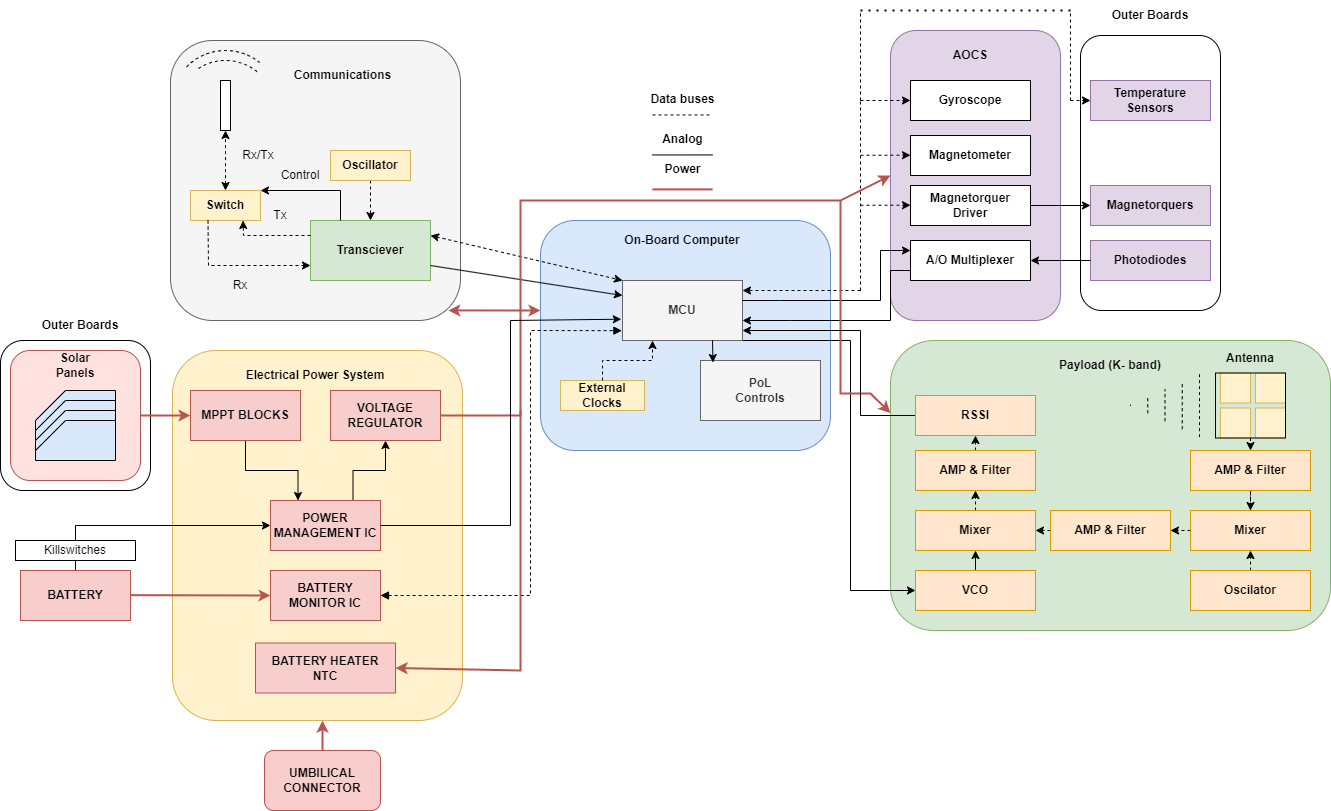
\includegraphics[width=0.8\linewidth]{res/img/1_introduction/1-PhysicalArchitectureBD.png}
    \caption{Physical architecture of $^{\text{Po}}$Cat 3 block diagram.}
    \label{fig:physarch-bd}
\end{figure}

\subsubsection{Communications (COMMS)}
The COMMS subsystem main fuctions are to receive and send data through radio
frequency (RF) waves. To do so it is provided of a monopole quarter-wavelenght
antenna, with an approximate lenght of 8.6cm, designed to transmit at 868MHz.
The signals to be sent by the spacecraft (telemetry) are generated and modulated 
by the transciever (combination of a radio transmitter and receiver). The signals
received are also demodulated at the transciever.

\paragraph{}

The system is half-duplex as radio information (transmission and reception) can
not be Tx'd and Rx'd at the same time. This is due to both the transicever 
capabilities and the use of a switch. The later regulates wether information 
is to be received or transmitted, and is controlled by the transciver itself
which is, at the same time, controlled bu the MCU. In fact, all transciver 
control is done by the MCU through a Serial Peripheral Interface (SPI).

\subsubsection{Electrical Power System (EPS) \& Power Generation}

The EPS subsystem manages power distribution and regulation.
Energy is obtained into the system through solar panels located 
at the lateral boards of the PocketQube. This energy is regulated 
by the MPPT blocks, one for each panel, and subministrated to the 
battery. Note that the killswitches ensure the satelite can't turn 
on when in it's rail before being deployed.
\paragraph{}
Power is distributed to the rest of the system after passing through 
the voltage regulator. A battery heater is located in this board. 
The heater ensures that the battery temperature is constrained to higher than 
it's lowest operating temperature and will be an object of interest in this report.
\paragraph{}
Finally, power can also be provided through the umbilical connector, still 
passing through the killswitches. The umbilical connector also allows code 
flashing into the MCU.

\subsubsection{On-Board Computer (OBC)}

The OBC subsystem's main component is the microcontroller unit (MCU). 
The MCU is in control of all data handling and on-board processing, 
acting as the brain of the spacecraft. Almost all information goes to 
or comes from the MCU and it is all stored there, either in its flash
memory or in its random access memory (RAM).
\paragraph{}
Physically, on the OBC board will also be located the COMMS subsystem as 
well as point of load (PoL) controls and external clocks to ensure the proper
 timing of the MCU.

\subsubsection{Attitude Determination and Control (ADCS)}

 The ADCS subsystem is the responsible for, as the name indicates, 
 attitude determination and control. To do so it is equipped with a 
 gyroscope, to measure it's angular velocity, a magnetometer to measure 
 the local magnetic field, the magnetorquer driver, which controls the 
 intensity that circulates through the magnetorquers, square, plain coils 
 located at the lateral boards that provide torque via electromagnetic 
 interactions, as well as an A/O Multiplexer that provides information 
 on sun position.
\paragraph{}
Temperature sensors are also placed on the lateral boards in order to 
provide insight for future missions, as a tumbling mode to avoid heat 
is not possible with the current architecture.

\subsubsection{K-Band (P/L)}
The payload on $^{\text{Po}}$Cat 3 measures RFI interference on the K-Band.
To do so it is equiped with a patch antenna, several amplifiers 
and filters as well as mixers, one regulated by an oscilator and
the other by a voltage controlled oscilator (VCO).

\subsubsection{L-Band (P/L)}
The payload on $^{\text{Po}}$Cat 2 measures RFI interference on the L-Band.
The main difference between both payloads is the antenna used, being in this case
a helicoidal deployable antenna.

\begin{figure}[H]
    \centering
    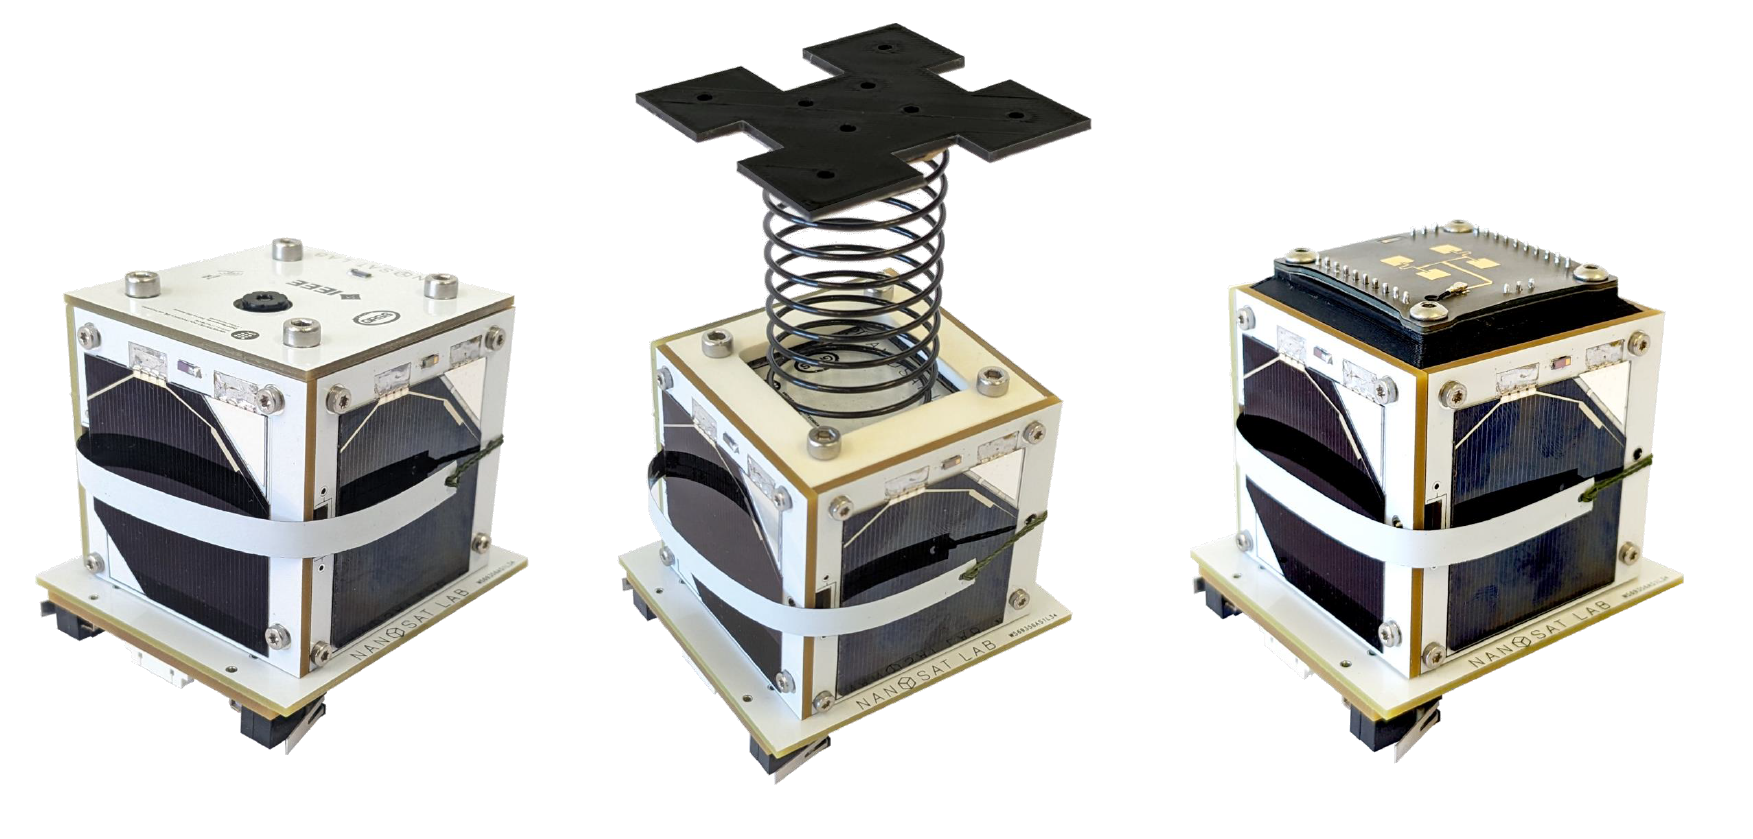
\includegraphics[width=0.8\linewidth]{res/img/1_introduction/pocat123.png}
    \caption{The $^{\text{Po}}$Cat 1,2,3 PocketQubes as of 2024.}
    \label{fig:pocat123}
\end{figure}


\subsection{Structure}

This project follows the PocketQube mechanical standard.
The satelite then, according to the 1P standard, consists of a 50 x 50 x 50 $mm^3$ cube,
placed onto a 64 x 58 $mm^2$ interface board, the latter acting as the mechanical 
interface between the satellite and the deployer pod. The contact is done by
having PCB edges represented in grey in the figure below slide into the
deployer rails, with the cube being fixed and later launched along the +Z 
direction. This interface board serves only the purpose described 
above. In the -Y direction, another PCB is mounted in order to house the 
circuitry correspondent to the ventral side of the cube.

\begin{figure}[H]
    \centering
    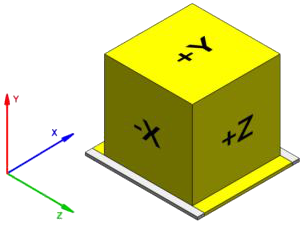
\includegraphics[width=0.4\linewidth]{res/img/1_introduction/Pqaxis.png}
    \caption{PocketQube reference frame.}
    \label{fig:pqaxis}
\end{figure}

The proposed solution for the inner structure is presented below:

\begin{figure}[H]
    \centering
    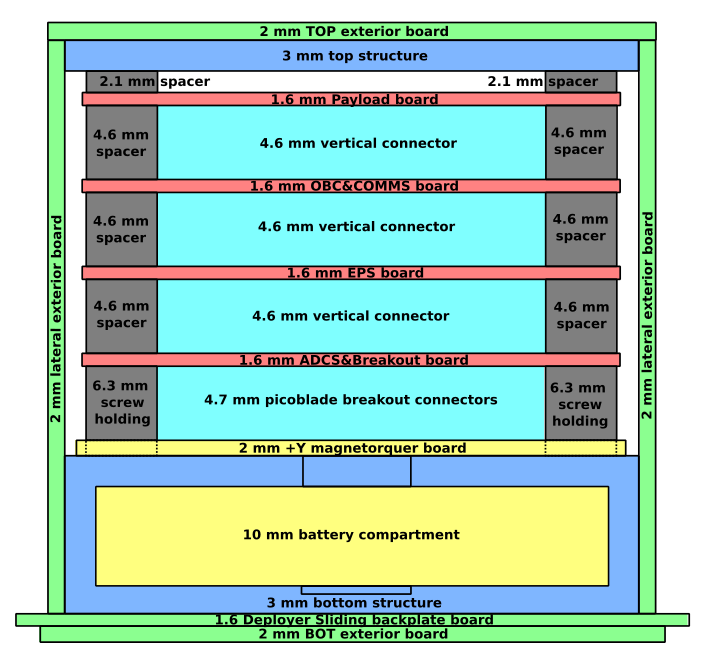
\includegraphics[width=0.4\linewidth]{res/img/1_introduction/2-GeneralStructure.png}
    \caption{Basic Structure of  the$^{\text{Po}}$Cat spacecraft.}
    \label{fig:genstruc}
\end{figure}

In \textbf{\textcolor{green}{green}}, we can see the outer boards, which form the
external part of the satellite. On the bottom exterior board, the 
killswitches are located, while the deployer sliding backplate will be the only PCB in
contact with the deployer rail. Consider that the top exterior board 
is subject to the payload used for each satellite. If the payload 
can be implemented on a single PCB (Payload board), this top exterior 
board remains in place. In the case of our payloads, both the K-Band
and the L-Band, the top exterior board is replaced by the payload board.

\paragraph{}

In \textbf{\textcolor{blue}{blue}}, we can see the only two internal structures 
that are not PCBs. The bottom structure will house the battery and act as an 
interface between the bottom exterior board and the sliding plate, connecting 
them with the rest of the subsystem stack. This structure will be made of PTFE
(Teflon). The top structure, made of 7075 Aluminium Alloy, will be used for 
the K-Band, acting as the interface between the payload and the rest of the 
subsystem stack. Additionally, both structures will allow the lateral boards 
to be screwed into them.

\paragraph{}

In \textbf{\textcolor{red}{red}}, we find the PCBs that form the various subsystems.
From top to bottom, these are: the Payload board (for the payload, additional PCBs 
may be added inside the payload), the OBC and COMMS board, the EPS board, and the 
ADCS board. These PCBs are connected to each other via the vertical connectors,
shown in \textbf{\textcolor{cyan}{cyan}}, which allow electrical interconnection 
between all the PCBs in the stack.
\paragraph{}

In \textbf{\textcolor{gray}{gray}}, spacers distribute the force from the 
tightened screws, preventing the vertical pins from bearing the full load.
\paragraph{}

Finally, in \textbf{\textcolor{yellow}{yellow}}, see the +Y magnetorquer and 
the battery.
\paragraph{}

More information on the materials is provided in its corresponding section. The K-Band
PQ structure:

\begin{figure}[H]
    \centering
    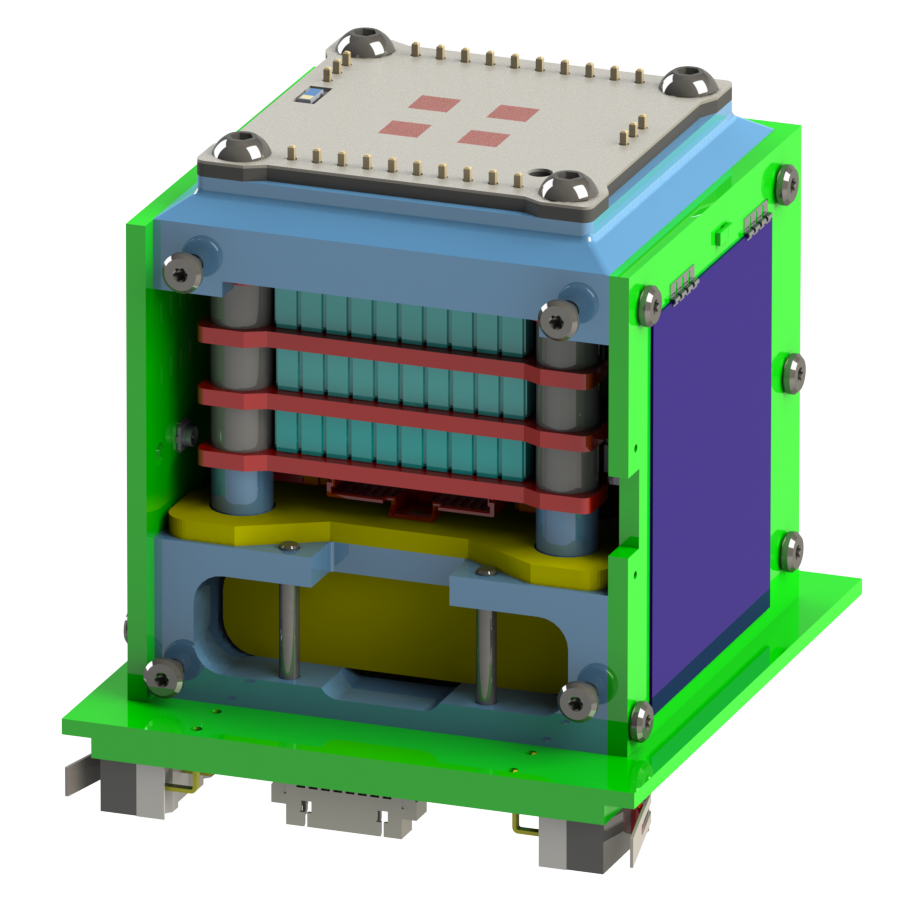
\includegraphics[width=0.3\linewidth]{res/img/1_introduction/3-KbandStrucColored.png}
    \caption{Colored K-Band PQ Structure}
    \label{fig:kbandstruc}
\end{figure}